\chapter{Evaluation und Ergebnisse}
In diesem Kapitel werden die Evaluation und die Ergebnisse von \textit{Reforge} vorgestellt. Es beginnt mit einer Beschreibung des Konfigurationsmanagements und der Inbetriebnahme von \textit{Reforge}. Anschließend werden die Kosten für die Nutzung der API analysiert. Die Qualität der generierten Berichte und die mobile Nutzbarkeit werden bewertet. Außerdem wird ein Vergleich der Anwendung \textit{Reforge} mit bestehenden Tools durchgeführt. Abschließend werden die wichtigsten Erkenntnisse und Erfahrungen aus dem Entwicklungsprozess zusammengefasst.

\section{Konfigurationsmanagement und Inbetriebnahme}

Um \textit{Reforge} lokal auszuführen, sind einige Vorbereitungen erforderlich. In diesem Abschnitt wird der Prozess der \ac{API}-Schlüsselgenerierung für OpenAI und DeepL sowie deren Integration in die Anwendung beschrieben.

\subsubsection{Was ist eine \texttt{.env}-Datei?}

Eine \texttt{.env}-Datei ist eine Umgebungsdatei. Sie dient dazu, sensible Konfigurationsdaten wie \ac{API}-Schlüssel, Datenbankzugangsdaten oder andere Umgebungsvariablen sicher zu speichern. Die Anwendung liest die \texttt{.env}-Datei beim Start aus, so dass diese Variablen nicht direkt im Code stehen müssen.

\subsubsection{Die \ac{API}-Schlüsselgenerierung}

Für die Nutzung der OpenAI- und DeepL-\ac{API}s müssen zunächst \ac{API}-Schlüssel generiert werden. Der Prozess beginnt mit der Erstellung eines Benutzerkontos bei den jeweiligen Plattformen. 

Für OpenAI wird die Website \href{https://platform.openai.com}{https://platform.openai.com} besucht, um sich anzumelden oder zu registrieren. Danach wird ein Dashboard sichtbar, über das eine Navigation zu den \ac{API} Keys möglich ist. Nachdem eine Zahlungsmethode hinterlegt wurde, kann dort über \textbf{Create new secret key} ein neuer Schlüssel generiert werden. Es ist wichtig, den Schlüssel direkt zu kopieren und sicher zu speichern, da er nur einmal angezeigt wird.

In ähnlicher Weise erfolgt die Schlüsselgenerierung für DeepL. Es wird die Webseite \href{https://www.deepl.com/pro}{https://www.deepl.com/pro} aufgerufen, um dort einen Account zu erstellen. Anschließend muss auch hier eine Zahlungsmethode ausgewählt werden, womit der Zugriff auf die \ac{API} ermöglicht wird. Im Bereich des Benutzerkontos gibt es einen \ac{API}-Bereich, in dem ein Schlüssel generiert werden kann. Auch hier sollte der Schlüssel sicher gespeichert werden, da er nur einmal erscheint und für die spätere Konfiguration der Anwendung benötigt wird.

\subsubsection{Integration der \ac{API}-Schlüssel in \textit{Reforge}}

Die \textit{Reforge}-Anwendung ist öffentlich auf GitHub verfügbar und kann lokal betrieben werden. Es ist über diesen Link erreichbar: \href{https://github.com/cyberlytics/reforge}{https://github.com/cyberlytics/reforge}

Das Repository muss zunächst in ein lokales Verzeichnis geklont werden. Im Verzeichnis \texttt{sys-src/backend} befindet sich die Datei \texttt{env-example}, die als Vorlage für die Konfiguration der \ac{API}-Schlüssel dient. Um die Anwendung betriebsbereit zu bekommen, müssen die in der Datei enthaltenen Platzhalter durch die zuvor generierten \ac{API}-Schlüssel ersetzt werden.

Der Platzhalter \textbf{dein-openai-api-schluessel} wird durch den \ac{API}-Schlüssel von OpenAI ersetzt, während \textbf{dein-deepl-api-schluessel} mit dem DeepL-Schlüssel überschrieben wird. Anschließend wird die Datei von \texttt{env-example} in \texttt{.env} umbenannt, sodass sie von der Anwendung korrekt eingelesen werden kann. Die resultierende \texttt{.env}-Datei sollte dann wie in Listing \ref{env-api-key} aussehen. Dabei handelt es sich hier um Beispiel-Keys, die nicht funktionsfähig sind und lediglich der Veranschaulichung dienen.

\begin{listing}[H]
\begin{minted}[
frame=lines,
bgcolor=base,
fontsize=\footnotesize,
linenos
]
{csharp}
    OPENAI_API_KEY=sk-12345abcdefghijklmnopqrstuvwxyz12345  
    DEEPL_API_KEY=12345678-90ab-cdef-1234-567890abcdef:fx
\end{minted}
\caption{\texttt{.env}-Datei im sys-src/backend-Ordner}
\label{env-api-key}
\end{listing}

\subsubsection{Inbetriebnahme der Anwendung}

Nachdem die \ac{API}-Schlüssel erfolgreich konfiguriert wurden, müssen die notwendigen Abhängigkeiten installiert werden. Dazu muss der Befehl \textbf{npm install} in einem Terminal in mehreren Verzeichnissen ausgeführt werden. Zuerst im Wurzelverzeichnis, dann im Verzeichnis \texttt{sys-src/backend} und schließlich im Verzeichnis \texttt{sys-src/frontend}. Dieser Schritt stellt sicher, dass alle für die Anwendung benötigten Pakete heruntergeladen und installiert werden.

Nach der Installation der Abhängigkeiten kann die Anwendung gestartet werden. Dazu wird im Terminal in das Verzeichnis \texttt{sys-src/backend} gewechselt und der Backend-Server mit dem Befehl \textbf{npm start} gestartet. Anschließend wird in das Verzeichnis \texttt{sys-src/frontend} navigiert und das Frontend ebenfalls mit \textbf{npm start} ausgeführt. Nach erfolgreichem Start der Anwendung öffnet sich automatisch die \textit{Reforge}-Oberfläche im Browser und steht für die Generierung von technischen Berichten zur Verfügung.

\subsubsection{Hinweise zu möglichen Problemen}

Bei der Nutzung der \textit{Reforge}-Anwendung können unter Umständen Probleme auftreten, die berücksichtigt werden sollten. Zum einen besteht die Möglichkeit, dass die \ac{API}s von OpenAI oder DeepL temporär ausfallen. Solche Ausfälle sind selten, sind aber während der Entwicklungszeit von \textit{Reforge} einmal aufgetreten. In solchen Fällen bleibt nichts anderes übrig, als auf die Behebung der Störung durch die jeweiligen Anbieter zu warten.

Andererseits ist zu beachten, dass die Nutzung der OpenAI-\ac{API} mit Kosten verbunden ist. Diese richten sich nach der Anzahl des verarbeiteten Tokens und variieren je nach Nutzungshäufigkeit und Größe der Anfragen. Eine Aufschlüsselung der entstehenden Kosten ist im folgenden Kapitel \ref{sec:apikosten} beschrieben.

\section{Kosten der API-Nutzung}
\label{sec:apikosten}

Für die Umsetzung der Anwendung wurden die OpenAI und DeepL \ac{API}s genutzt. Die Nutzung dieser \ac{API}s sind mit unterschiedlichen Kosten verbunden, die hier näher erläutert werden.

Die OpenAI \ac{API} bietet verschiedene Preismodelle an, welche auf der Anzahl der verwendeten Tokens basieren. Die Kosten richten sich nach der Anzahl der Ein- und Ausgabe-Token, wobei pro 1.000 Token ein bestimmter Betrag berechnet wird. Für dieses Projekt wurde das \ac{GPT}-3.5-turbo Modell verwendet und zum Zeitpunkt der Entwicklung betrugen die Kosten für \ac{GPT}-3.5-turbo ca. 0,002 US-Dollar pro 1.000 Token. Die tatsächlichen Kosten können je nach Umfang der Anfragen variieren, da längere Dokumente und komplexere Anfragen zu einer höheren Anzahl von Token führen.

Die Abbildung \ref{fig:OpenAI Kosten} zeigt ein Diagramm, welches die Kosten der OpenAI \ac{API} für den Monat August im Jahr 2024 darstellt. Dabei handelt es sich um eine Webseite, auf die zugegriffen werden kann, sobald eine OpenAI \ac{API} verwendet wird. Die Balken, die in der Abbildung zu sehen sind, sind während der Entwicklung von \textit{Reforge} entstanden, als die Anwendung mit Testdaten ausprobiert wurde. Diese Daten können jedoch für eine vorausschauende Kostenanalyse genutzt werden.

\begin{figure}[H]
\centering
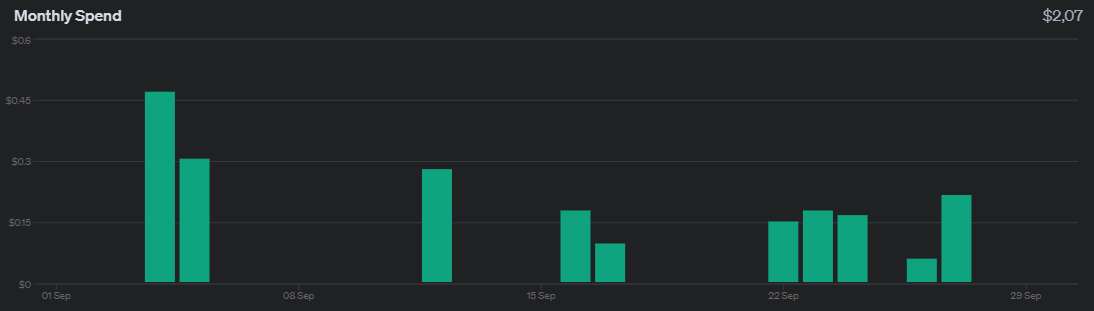
\includegraphics[width=1\linewidth]{Images/MonthlySpend.png}\\
\caption{OpenAI Kosten von August}
\label{fig:OpenAI Kosten}
\end{figure}

Ein weiteres nützliches Diagramm ist in Abbildung \ref{fig:OpenAI Token Usage} dargestellt, welches die Input Tokens und Output Tokens in Relation zu den Kosten zeigt. Aus dem Diagramm geht hervor, dass es sich um Zusammenfassungen handelt, da die Balken für die Output Tokens einen geringeren Ausschlag als die Input Tokens haben. 

\begin{figure}[H]
\centering
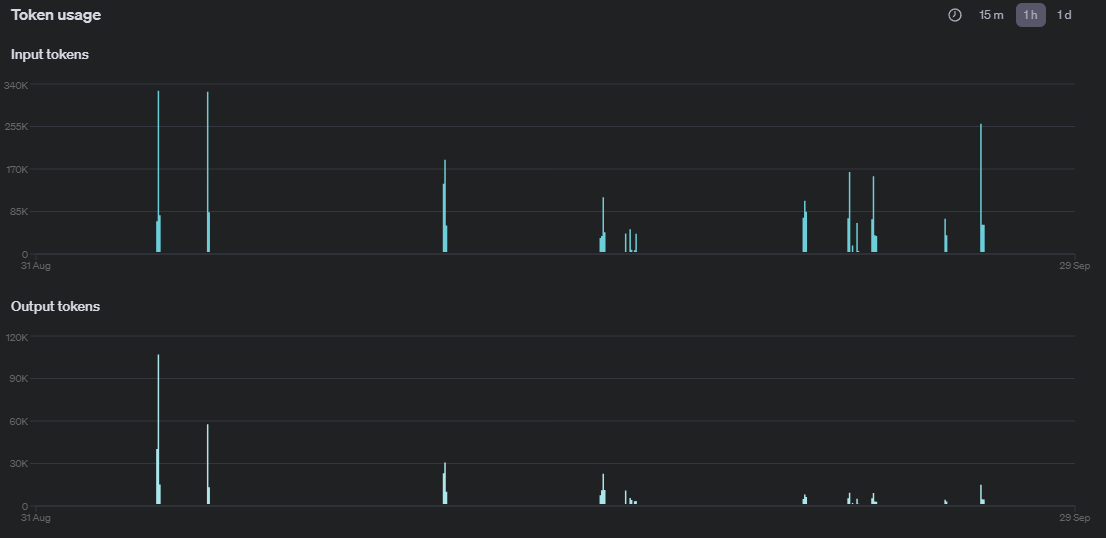
\includegraphics[width=1\linewidth]{Images/TokenUsage.png}\\
\caption{OpenAI Token Usage von August}
\label{fig:OpenAI Token Usage}
\end{figure}

Für den gesamten Entwicklungszeitraum beliefen sich die Kosten für OpenAI auf insgesamt 2,68 US-Dollar. Im August betrugen die Kosten 0,41 US-Dollar, im September 2,07 US-Dollar und im Oktober 0,20 US-Dollar. Insgesamt wurden 118 Berichte generiert, was einem Durchschnitt von ca. 0,023 US-Dollar pro Bericht entspricht. Der Tokenverbrauch zeigt, dass größere Berichte mehr Token und damit höhere Kosten verursachen, während kürzere Dokumente weniger Ressourcen beanspruchen.

Für die DeepL \ac{API} wurde die kostenlose Version verwendet. Diese Version erlaubt eine begrenzte Anzahl an Übersetzungen pro Monat, bietet jedoch eine ausreichende Qualität für die Anforderungen dieses Projekts. Die kostenlose Version ist ideal für kleinere Projekte, da keine direkten Kosten entstehen und dennoch hochwertige Übersetzungen zwischen Deutsch und Englisch möglich sind. Bei einem größeren Umfang oder einer intensiveren Nutzung könnte jedoch eine kostenpflichtige Version erforderlich werden, die zusätzliche Funktionen und ein höheres Übersetzungslimit bietet.

Die Kosten der verwendeten \ac{API}s sind insgesamt überschaubar, insbesondere da die kostenlose Version von DeepL genutzt werden kann. Die OpenAI \ac{API} hingegen verursacht Kosten, die jedoch im Rahmen bleiben und durch die Qualität der generierten Zusammenfassungen gerechtfertigt werden können. Für zukünftige Projekte könnte gegebenenfalls die Nutzung eines anderen OpenAI Modells sinnvoll sein, um das Kosten-Nutzen-Verhältnis weiter zu optimieren.

\section{Qualität der generierten Berichte}

Um die Qualität der erstellten Berichte zu bewerten, wurde ein Bericht auf der Grundlage dieser Arbeit mit \textit{Reforge} produziert. Für die LaTeX-Ausgabe wurde der Bericht in englischer Sprache generiert. Das Ergebnis dieser Generierung ist im Anhang in den Abbildungen \ref{fig:Reforge_testgen1} und \ref{fig:Reforge_testgen2} dargestellt. Zusätzlich wurde eine Generierung für die \ac{DOCX}-Ausgabe durchgeführt. Die Ergebnisse dieser Ausgabe sind ebenfalls im Anhang unter den Abbildungen \ref{fig:ReforgeDOCXGen1} und \ref{fig:ReforgeDOCXGen2} zu finden.

Wie Chang et al. in ihrer Evaluation von \ac{LLM}s beschreiben, neigen \ac{LLM}s in komplexen Kontexten zu Verwechslungen oder Fehlern. Sie stoßen bei der Erkennung semantischer Ähnlichkeiten an ihre Grenzen und zeigen Schwächen in ressourcenarmen Kontexten \cite{10.1145/3641289}. Ob diese Einschränkungen auch hier zutreffen, wurde überprüft. Es zeigte sich, dass Schwächen in ressourcenarmen Kontexten erkennbar sind. Betrachtet man die Abschnitte Bilder und Codeauszüge in den Abbildungen \ref{fig:Reforge_testgen2} und \ref{fig:ReforgeDOCXGen2}, so fällt ein Mangel an Inhalt auf. Dies ist darauf zurückzuführen, dass in diesen Abschnitten kein Text vorhanden ist. Die \textit{Reforge}-Anwendung verarbeitet derzeit keine Bilder und Codeausschnitte, wodurch dieser ressourcenarme Kontext entsteht.

Um die Kompressionsrate $\tau$ von Yadav zu berechnen, wurde die Anzahl der Wörter berücksichtigt \cite{yadav2022automatictextsummarizationmethods}. Diese Arbeit enthält ungefähr 24.150 Wörter. Die Anzahl der Wörter in der generierten \ac{DOCX}-Zusammenfassung \ref{fig:ReforgeDOCXGen1} beträgt ungefähr 970 Wörter. Mit diesen Werten kann nun die Kompressionsrate berechnet werden.

\begin{align}
\mathlarger{\text{0,04017} = \frac{| \text{970} |}{| \text{24.150} |}}
\end{align}

Die Kompressionsrate beträgt somit gerundet 4\% und liegt damit weit unter den gewünschten 15-30\%, die Yadav als gut erachtet. Dies lässt den Schluss zu, dass entweder \textit{Reforge} zu viel Inhalt entfernt oder \ac{GPT}-3.5-turbo zu viel Information auslässt.

Es werden nun die gestellten Fragen aus der Einleitung \ref{einleitung} betrachtet. Zunächst wird untersucht, ob in den generierten Inhalten Biases auftreten. Es zeigt sich, dass das \ac{GPT}-3.5-turbo-Modell keine Biases in den generierten Inhalten aufweist, da es sich ausschließlich auf den Inhalt des hochgeladenen Dokuments stützt.

Die zweite Frage beschäftigt sich damit, ob \textit{Reforge} mithilfe von \ac{KI} bessere Ergebnisse erzielt als ein Mensch. Hier wird deutlich, dass \textit{Reforge} in der Lage ist, eine solide Grundlage zu schaffen. Diese Ergebnisse müssen jedoch von einem Menschen überarbeitet und geprüft werden, sodass \textit{Reforge} die Arbeit des Menschen nicht vollständig ersetzt, sondern lediglich unterstützt.

Abschließend wurde die Frage betrachtet, inwieweit sich die Input-Datei im Vergleich zur Output-Datei verändert. Es konnte festgestellt werden, dass die grobe Inhaltsstruktur erhalten bleibt, während Details teilweise ausgelassen werden. Die weitere Bewertung des erstellten Berichts erfolgte anhand folgender Kriterien.

\begin{itemize}
    \item \textbf{Inhaltliche Genauigkeit:} Die erstellten Zusammenfassungen wurden auf ihre inhaltliche Richtigkeit überprüft. Dabei wurde geprüft, ob die wesentlichen Informationen des Originaldokuments korrekt in die Zusammenfassung übernommen wurden. Die Ergebnisse zeigen, dass das \ac{LLM} in der Lage ist, die wichtigsten Inhalte zusammenzufassen. Da es sich jedoch um eine komprimierte Fassung handelt, gehen Informationen hinsichtlich der Erläuterung der Inhalte verloren.
    \item \textbf{Kohärenz und Lesbarkeit:} Die Berichte sind im Allgemeinen gut lesbar und logisch aufgebaut. Die Verwendung von \ac{LLM} trägt dazu bei, dass die Texte eine natürliche Sprache aufweisen. Dennoch gibt es vereinzelte Fälle, in denen Sätze etwas zu komplex formuliert sind, was die Lesbarkeit beeinträchtigen könnte.
    \item \textbf{Formatierung und Layout:} Ein weiterer wichtiger Aspekt der Evaluierung ist die Formatierung und das Layout der Berichte. Die Anwendung ist in der Lage, vorgegebene Vorlagen wie LaTeX oder \ac{DOCX} korrekt umzusetzen, so dass die resultierenden Berichte den Anforderungen der jeweiligen Vorlage entsprechen.
    \item \textbf{Übersetzungsqualität:} Bei der Evaluierung der Übersetzungsfunktion wurde die Qualität der Übersetzung des generierten LaTeX-Berichts zwischen Deutsch und Englisch untersucht. Das \ac{GPT}-3.5-turbo-Modell erwies sich als zuverlässig. Die Übersetzungen sind im Allgemeinen korrekt und behalten die ursprüngliche Bedeutung des Inhalts bei. Die Titelübersetzungen von DeepL sind ebenfalls richtig.
    \item \textbf{Geschwindigkeit:} Die Erstellung der technischen Berichte dauerte immer weniger als eine Minute und ist somit ein schneller Prozess. Der Zeitaufwand für die Generierung ist im Vergleich zu manuellen Zusammenfassungen minimal.
\end{itemize}

Insgesamt wurde die Qualität der erstellten Berichte als gut bewertet. Die Anwendung erzeugt verständliche technische Berichte und ermöglicht eine korrekte Formatierung. Sie bietet eine gute Vorlage, die manuell ergänzt werden kann.

\section{Evaluation der mobilen Ansicht von \textit{Reforge}}

Die mobile Ansicht der \textit{Reforge}-Anwendung wurde im Browser getestet, um ihre Nutzbarkeit auf kleineren Bildschirmen zu bewerten. Obwohl sich die Webseite für mobile Geräte automatisch skaliert, treten vereinzelt kleinere Layout-Probleme auf. Diese beeinträchtigen jedoch nicht die Funktionalität der Anwendung, sodass die Seite weiterhin vollständig nutzbar bleibt. Die Darstellung der mobilen Version ist in Abbildung \ref{fig:MobileRefUP} zu sehen. \textit{Reforge} erfüllt somit die Anforderungen an Responsive Design. 

\begin{figure}[H]
\centering
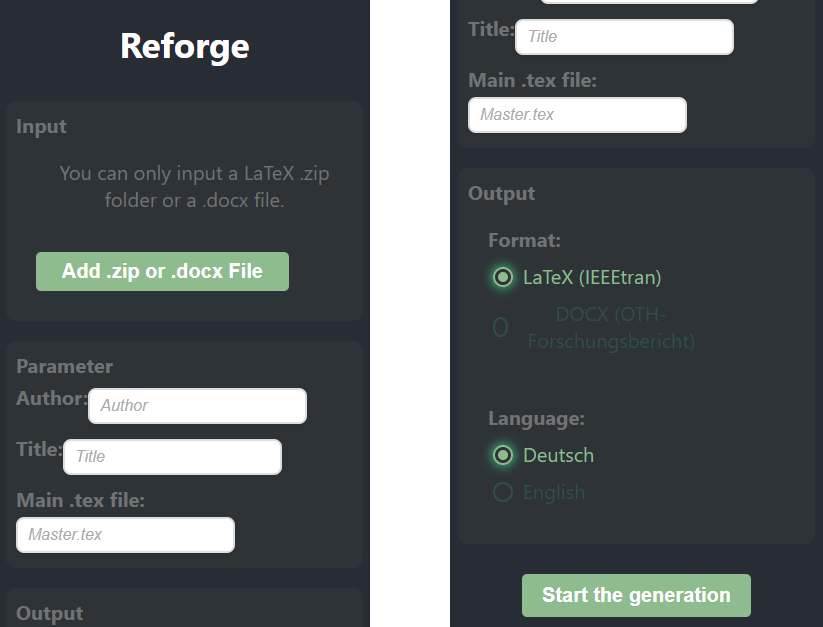
\includegraphics[width=0.8\linewidth]{Images/MobileReforge.png}\\
\caption{Die mobile Ansicht der Upload-Seite von \textit{Reforge}}
\label{fig:MobileRefUP}
\end{figure}

\section{Projektvergleich mit verwandten Webanwendungen}
Um herauszufinden, ob die bestehenden Werkzeuge besser sind als \textit{Reforge}, wird in diesem Abschnitt ein Vergleich mit den verwandten Webanwendungen durchgeführt. Dies soll helfen, den Nutzen von \textit{Reforge} besser einschätzen zu können. 

\subsection{Vergleich mit ChatGPT-4}
Für diesen Vergleich wird versucht, die mit \textit{Reforge} möglichen Ausgaben mit Chat\ac{GPT} zu erzeugen. Dazu wird Chat\ac{GPT} als Eingabe entweder ein \ac{DOCX}-Dokument oder ein LaTeX-ZIP-Ordner übergeben. Zusätzlich wird ein Prompt angegeben, der Chat\ac{GPT} anweist, einen technischen Bericht zu erzeugen. Außerdem wird das Ausgabeformat angegeben, in dem der Bericht erzeugt werden soll. Ähnlich wie bei \textit{Reforge} wird für die LaTeX-Ausgabe IEEEtran und für das \ac{DOCX}-Dokument der OTH-Forschungsbericht angefordert. Um jede Kombination einmal zu testen, werden vier Tests benötigt. Die Ergebnisse der einzelnen Tests sind unten aufgeführt.  Als LaTeX-ZIP-Testdokument für die Generierung wurde die Bachelorarbeit von Hoffmann verwendet \cite{hoffmann_tim_2022bt}. Die Bachelorarbeit von Schotter wurde als Testdokument für die \ac{DOCX}-Generierung verwendet \cite{schotter_tobias_2022bt}.

\subsubsection{Test 1 - LaTeX-ZIP-Ordner zu LaTeX}

Für diesen Vergleich wurde Chat\ac{GPT} gebeten, aus dem LaTeX-ZIP-Archiv eine LaTeX-Ausgabe zu erzeugen. In der Abbildung \ref{fig:Zip_test_anfrage} ist der übergebene Test-Prompt zu sehen. Mit diesem Prompt wurde versucht, Chat\ac{GPT} dazu zu bringen, aus der LaTeX-ZIP-Datei einen technischen Bericht im IEEEtran-Format zu erstellen.

\begin{figure}[H]
\centering

\includegraphics[width=0.8\linewidth]{Images/Zip_test_anfrage.png}\\
\caption{ZIP-Test-Prompt an ChatGPT}
\label{fig:Zip_test_anfrage}
\end{figure}

Chat\ac{GPT} war jedoch nach mehrmaliger Aufforderung nicht in der Lage, das ZIP-Archiv zu analysieren und das gewünschte Ergebnis zu liefern. Es wurde lediglich auf den Inhalt der LaTeX-ZIP-Datei eingegangen und erwähnt, dass die Inhaltsanalyse in Arbeit sei. Die Antwort auf den Prompt ist in der Abbildung \ref{fig:Zip_test_antwort} dargestellt.

\begin{figure}[H]
\centering

\includegraphics[width=0.9\linewidth]{Images/Zip-test-antwort.png}\\
\caption{ZIP-Test-Antwort von Chat\ac{GPT}}
\label{fig:Zip_test_antwort}
\end{figure}

\subsubsection{Test 2 - DOCX zu LaTeX}

In einem weiteren Test wurde nun das \ac{DOCX}-Dokument an Chat\ac{GPT} übergeben. Dabei war Chat\ac{GPT} in der Lage, eine LaTeX-Ausgabe zu erzeugen, die auch das IEEEtran-Format darstellt. Ein auffallender Nachteil ist jedoch der fehlende Download-Button. Mit Chat\ac{GPT} muss der erzeugte Text manuell kopiert und in eine LaTeX-Datei konvertiert werden, was für den Benutzer zusätzliche Umstände mit sich bringt. Die Chat\ac{GPT} Antwort ist in der Abbildung \ref{fig:docxzulatexgpt} im Anhang dargestellt.

Darüber hinaus gibt es kleinere Fehler in der Ausgabe, wie zum Beispiel die Vermischung von deutscher und englischer Sprache und das Fehlen des Inhalts des Reference-Abschnitts. Dieser Abschnitt müsste bei Bedarf manuell eingefügt werden. Außerdem wurde eine Beispiel-E-Mail eingefügt, die ebenfalls im Nachhinein angepasst werden müsste. Das generierte Ergebnis von Chat\ac{GPT} ist im Anhang in der Abbildung \ref{fig:docxzulatexresult} zu sehen.


\subsubsection{Test 3 - LaTeX-ZIP-Ordner zu \ac{DOCX}}

Es wurde versucht, eine \ac{DOCX}-Ausgabe aus dem LaTeX-ZIP-Ordner zu erhalten. Dazu wurde Chat\ac{GPT} angewiesen, einen technischen Bericht für \ac{DOCX} zu erzeugen. Bei diesem Test erzeugte Chat\ac{GPT} einen Download-Link, um das erstellte \ac{DOCX}-Dokument herunterzuladen. Die Chat\ac{GPT} Antwort auf diesen Test ist in der Abbildung \ref{fig:latexzudocxgpt} im Anhang dargestellt.  

Bei näherer Betrachtung wies das von Chat\ac{GPT} erstellte Dokument zahlreiche Fehler auf, wie die Abbildung \ref{fig:latexzudocxresult} im Anhang zeigt. Die Kapitel sind nicht benannt, sondern durchnummeriert. Außerdem fehlt der obere Rahmen mit Titel, Autor und Studiengang. Ein weiterer Fehler ist, dass LaTeX-Befehle wie Chapter, Section, Cite, Label und Begin im Text vorkommen. Schließlich fehlt der Inhalt des Referenzteils.  

\subsubsection{Test 4 - \ac{DOCX} zu \ac{DOCX}}

Im vierten Test wird probiert, aus dem \ac{DOCX}-Dokument eine \ac{DOCX} Zusammenfassung zu erzeugen. Es wird festgestellt, dass der obere Rahmen wie Autor, Studiengang, Hochschule und Ort fehlt. Außerdem gibt es auch hier keine Referenzsektion. Ein weiteres Problem ist, dass die Ausgabe manuell in eine \ac{DOCX}-Datei eingefügt werden muss. Wie die Chat\ac{GPT}-Ausgabe aussieht, ist im Anhang unter \ref{fig:docxzudocx} zu finden.

\subsubsection{Schlussfolgerung}

Zusammengefasst ist nur Test zwei auf einem ähnlichen Niveau wie die Ausgabe in \textit{Reforge}. Allerdings muss der Benutzer im Dokument von Test zwei die Sprache, die Referenzen und die Daten wie E-Mail überprüfen oder ändern. Alle anderen Tests weisen zu viele Mängel auf, die durch den Anwender korrigiert werden müssten. Andererseits ist anzumerken, dass durch eine Änderung des Prompts möglicherweise bessere Ergebnisse erzielt werden könnten.

Im Vergleich zu Chat\ac{GPT} bietet \textit{Reforge} eine konsistente Ausgabe in Bezug auf Layout und Export. Außerdem muss sich der Benutzer nicht um einen eigenen Prompt bemühen. Er muss lediglich seine Dokumente hochladen und die gewünschten Parameter auswählen. Darüber hinaus achtet \textit{Reforge} auf die Textsprache, so dass es nicht vorkommen kann, dass im Endprodukt eine Mischung aus Englisch und Deutsch erscheint. 

\subsection{Vergleich mit Copilot}
Bei diesem Vergleich wurde zunächst versucht, ein \ac{DOCX}-Dokument in Copilot hochzuladen. Dies wurde jedoch von Copilot mit der Meldung abgelehnt, dass nur Bilder hochgeladen werden können. Diese Mitteilung ist in Abbildung \ref{fig:Copilot_File} dargestellt.

\begin{figure}[H]
\centering

\includegraphics[width=0.7\linewidth]{Images/Copilot_File.png}\\
\caption{Copilot Datei Einschränkungen}
\label{fig:Copilot_File}
\end{figure}

Da ein direktes Hochladen der Datei nicht möglich war, wurde alternativ der Inhalt des \ac{DOCX}-Dokuments kopiert und eingefügt. Dabei stellte sich heraus, dass Copilot ein Zeichenlimit von 10.240 Zeichen vorgibt. Dies ist problematisch, da wissenschaftliche Arbeiten in der Regel deutlich umfangreicher sind. Diese Beschränkung ist in Abbildung \ref{fig:Copilot_Limit} dargestellt. Um Copilot dennoch als Werkzeug für die Berichterstellung nutzen zu können, wäre es notwendig, den Text manuell in kleinere Abschnitte zu unterteilen und diese einzeln zu bearbeiten. Dies würde jedoch einen erheblichen Mehraufwand für den Anwender bedeuten.  

\begin{figure}[H]
\centering

\includegraphics[width=1\linewidth]{Images/Copilot_Limit.png}\\
\caption{Copilot Textlängen Limitierung}
\label{fig:Copilot_Limit}
\end{figure}

Abschließend lässt sich festhalten, dass \textit{Reforge} gegenüber Copilot den Vorteil bietet, dass Dokumente direkt hochgeladen werden können und die Inhalte automatisch in bearbeitbare Abschnitte unterteilt werden. Zudem muss der Benutzer bei \textit{Reforge} keine eigenen Prompts erstellen, da diese bereits vordefiniert sind. Dies vereinfacht die Anwendung und reduziert den Arbeitsaufwand.

\subsection{Vergleich mit Gemini}
Als drittes Vergleichstool wurde Gemini ausgewählt. Ähnlich wie bei Copilot ist das Hochladen von Dateien in Gemini eingeschränkt, wie in Abbildung \ref{fig:Copilot_File} dargestellt. Außerdem muss der Benutzer bei Gemini zusätzlich einen entsprechenden Prompt für die Verarbeitung angeben.

\begin{figure}[H]
\centering

\includegraphics[width=1\linewidth]{Images/Gemini_File.png}\\
\caption{Gemini Datei Einschränkungen}
\label{fig:Gemini_File}
\end{figure}

Stattdessen wurde erneut versucht, den Textinhalt manuell in den Chat einzufügen. Auch hier gibt es jedoch eine Zeichenbegrenzung, ab der das Einfügen weiterer Inhalte nicht mehr möglich ist. Gemini zeigt allerdings keine genauen Informationen über die Zeichenbegrenzung an, was die Arbeit mit längeren Texten erschwert. Um den gesamten Inhalt eines Dokuments verarbeiten zu können, wäre es daher notwendig, den Text manuell in kleinere Abschnitte zu unterteilen.

Im Vergleich zu Gemini zeigt sich, dass der direkte Datei-Upload von \textit{Reforge} den Benutzern viele Arbeitsschritte erspart. Der Textinhalt wird in \textit{Reforge} automatisch in bearbeitbare Abschnitte unterteilt und es sind keine zusätzlichen Eingabeaufforderungen erforderlich.

\subsection{Vergleich mit QuillBot}
Zuletzt wurde \textit{Reforge} mit QuillBot verglichen, einem Tool, das wie \textit{Reforge} keine Chatfunktion bietet. Es dient lediglich zum Zusammenfassen von Texten und unterstützt daher nicht das direkte Hochladen von Dokumenten. Aus diesem Grund muss der Inhalt einer wissenschaftlichen Arbeit für die Zusammenfassung manuell kopiert und eingefügt werden. Es wurde jedoch festgestellt, dass QuillBot eine Begrenzung der Textlänge besitzt, die in Abbildung \ref{fig:Quillbot_Limit} dargestellt ist. Dieses Limit kann durch das Anlegen eines Accounts oder den Erwerb einer Premium-Mitgliedschaft erhöht werden. Diese Abbildung zeigt auch, dass die Zusammenfassung durch die Auswahl von Schlüsselwörtern personalisiert werden kann.  

\begin{figure}[H]
\centering
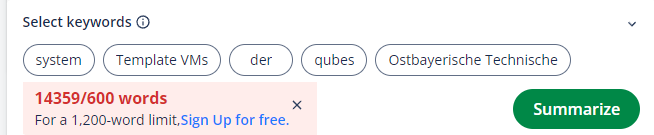
\includegraphics[width=0.8\linewidth]{Images/Quillbot_Limit.png}\\
\caption{Quillbot Textlängen Limitierung}
\label{fig:Quillbot_Limit}
\end{figure}

Weitere Einstellungen, wie beispielsweise die Länge der Zusammenfassung, können ebenfalls in QuillBot vorgenommen werden. Eine Übersicht dieser Einstellungsmöglichkeiten ist in Abbildung \ref{fig:Quillbot_Modes} dargestellt.

\begin{figure}[H]
\centering

\includegraphics[width=0.8\linewidth]{Images/Quillbot_Modes.png}\\
\caption{Quillbot Einstellugen für die Zusammenfassung}
\label{fig:Quillbot_Modes}
\end{figure}

Zusammenfassend lässt sich festhalten, dass QuillBot aufgrund der Beschränkung der Textlänge nicht mit \textit{Reforge} mithalten kann. Zudem fehlt die Möglichkeit, Dokumente direkt hochzuladen, was eine manuelle Eingabe des Textinhalts erfordert. Andererseits bieten die zusätzlichen Zusammenfassungsoptionen von Quillbot interessante Ansätze. Beispielsweise könnte die Anpassung der Zusammenfassungslänge für zukünftige Versionen von \textit{Reforge} in Betracht gezogen werden.

\section{Lessons Learned}

Die aus Projekten gewonnenen Erkenntnisse werden als Lessons Learned bezeichnet. Patton betrachtet Lessons Learned als lokales, erfahrungsbasiertes Wissen, das oft unspezifisch und ungeprüft ist. Er diskutiert, dass Lessons Learned nicht nur als Methode der Programmevaluierung verwendet werden sollten, sondern auch als Wissensquelle für eine effektive Programmgestaltung \cite{patton2001evaluation}. Im Folgenden wird daher auf die Erkenntnisse eingegangen, die zur Verbesserung zukünftiger Programmkonzeptionen genutzt werden können:

\begin{itemize}
    \item \textbf{Technische Herausforderungen und Lösungsansätze:} Die Integration der OpenAI \ac{API} erwies sich als technisch anspruchsvoll. Dies gilt insbesondere für die Optimierung der Token-Nutzung, um die Kosten gering zu halten. Es wurde gelernt, dass eine sorgfältige Planung der Abfragen und die Aufteilung langer Texte entscheidend ist, um die Tokenbeschränkungen einzuhalten.
    \item \textbf{Bedeutung der Benutzerfreundlichkeit:} Ein weiterer wichtiger Aspekt war die Gestaltung der Benutzeroberfläche. Die Gestaltungsprinzipien erwiesen sich als hilfreich, um die Anwendung auch für Nutzer ohne tiefere technische Kenntnisse zugänglich zu machen. Es wurde deutlich, dass eine klare und einfache Benutzerführung den Umgang mit der Anwendung erleichtert.
    \item \textbf{Kostenmanagement und \ac{API}-Nutzung:} Die monatlichen Kosten für die OpenAI \ac{API} waren überschaubar. Das Projekt hat jedoch gezeigt, dass eine genaue Kostenüberwachung und eine Beschränkung der Anfragen notwendig sind, um im vorgegebenen Budget zu bleiben. Die Nutzung der kostenlosen Version von DeepL war dabei eine sinnvolle Entscheidung, um die Kosten gering zu halten.
    \item \textbf{Zukunftspotenzial:} Während der Entwicklung wurde deutlich, dass die Anwendung durch die Integration weiterer Funktionen noch verbessert werden kann. Diese Erweiterungen bieten Potenzial für zukünftige Projekte und könnten die Anwendungsbreite und den Nutzen von \textit{Reforge} weiter ausbauen. In Kapitel \ref{ch:ausblick} werden mögliche Projekterweiterungen erläutert.
    \item \textbf{Zeitplanung:} Eine gute Zeitplanung ist für die Entwicklung von Anwendungen unerlässlich. Daher ist es wichtig, im Voraus zu überlegen, wie viel Zeit für welche Funktionen aufgewendet werden soll.
\end{itemize}

Die gewonnenen Erkenntnisse bieten wertvolle Einblicke, die in zukünftigen Projekten genutzt werden können.